\documentclass[12pt]{article}

\usepackage[utf8]{inputenc} % allow utf-8 input
\usepackage[T1]{fontenc}    % use 8-bit T1 fonts
\usepackage{hyperref}       % hyperlinks

% tables
\usepackage{longtable}
\usepackage{booktabs}
\usepackage{multirow}

% floats
\usepackage{caption}
\usepackage{subcaption}
\usepackage{graphicx}

% math
\usepackage{amsfonts,amsmath,amssymb}
\usepackage{nicefrac}

\renewcommand{\Pr}{\operatorname{Pr}}
\newcommand{\E}{\ensuremath{\operatorname{E}}}
\newcommand{\V}{\operatorname{V}}
\newcommand{\solve}[1]{\operatornamewithlimits{solve:\ }_{#1}}
\newcommand{\st}{\operatorname{subject\ to:\ }}
\newcommand{\argmin}[1]{\operatornamewithlimits{argmin:\ }_{#1}}
\newcommand{\argmax}[1]{\operatornamewithlimits{argmax:\ }_{#1}}
\newcommand{\etal}{\textit{et~al.}}

\newcommand{\CP}{\ensuremath{\operatorname{CP}}}
\newcommand{\ACP}{\ensuremath{\operatorname{ACP}}}
\newcommand{\OCP}{\ensuremath{\operatorname{OCP}}}
\newcommand{\PP}{\ensuremath{\operatorname{PP}}}
\newcommand{\EP}{\ensuremath{\operatorname{EP}}}
\renewcommand{\Pr}{\ensuremath{\operatorname{Pr}}}
\newcommand{\cond}{\ensuremath{\,|\,}}
%\newcommand{\c}{\ensuremath{z_{1-\alpha}}}


% other
\usepackage{color}
\usepackage{hyperref}
\usepackage[numbers,super,sort&compress]{NJDnatbib}
\bibliographystyle{WileyNJD-AMA}
\usepackage{scalerel}
\newcommand{\kr}[1]{{\color{red}#1}}
\usepackage{comment}


\title{Conditional Power and Friends: The Why and How of (Un)planned, Unblinded Sample Size Recalculations in Confirmatory Trials}

\author{
    \footnotesize Kevin Kunzmann\\
    \footnotesize MRC Biostatistics Unit, University of Cambridge \\
    \footnotesize
    East Forvie Building, Robinson Way,
    Cambridge Biomedical Campus \\
    \footnotesize Cambridge CB2 0SR,
    United Kingdom \\
    \footnotesize \texttt{kevin.kunzmann@mrc-bsu.cam.ac.uk}
    \and
    \footnotesize Michael J. Grayling \\
    \footnotesize Population Health Sciences Institute, Newcastle University
    \and
    \footnotesize Kim May Lee \\
    \footnotesize Institute of Psychiatry, Psychology and Neuroscience, King's College London
    \and
    \footnotesize David S.\ Robertson \\
    \footnotesize MRC Biostatisics Unit, University of Cambridge
    \and
    \footnotesize Kaspar Rufibach \\
    \footnotesize Methods, Collaboration, and Outreach Group (MCO) \\
    \footnotesize Department of Biostatistics, F. Hoffmann-La Roche, Basel
    \and
    \footnotesize James M. S. Wason \\
    \footnotesize Population Health Sciences Institute, Newcastle University and \\
    \footnotesize MRC Biostatistics Unit, University of Cambridge
}


\usepackage{setspace}
\onehalfspacing
\pdfminorversion=4

\begin{document}

\maketitle

\captionsetup{width=\textwidth}

%\newpage
%\section*{Funding}
%\noindent
%David S. Robertson was funded by the Biometrika Trust and the Medical Research %Council under Grant MC\_UU\_00002/6.

\newpage

\begin{abstract}
Adapting the final sample size of a trial to the evidence accruing
during the trial is a natural way to address planning uncertainty.
Since the sample size is usually determined by an
argument based on the power of the trial,
an interim analysis raises the question of
how the final sample size should be determined conditional on the accrued information.
To this end, we first review and compare common approaches to estimating conditional power
which is often used in heuristic sample size recalculation rules.
We then discuss the connection of heuristic sample size recalculation and
optimal two-stage designs demonstrating that the latter is the superior approach in a fully pre-planned setting.
Hence, unplanned design adaptations should only be conducted
as reaction to trial-external new evidence, operational needs to violate the originally chosen design,
or \textit{post~hoc} changes in the optimality criterion but not as a reaction to trial-internal data.
We are able to show that commonly discussed sample size recalculation rules lead to paradoxical adaptations
where an initially planned optimal design is not invariant under the adaptation rule
even if the planning assumptions do not change.
Finally, we propose two alternative ways of reacting to
newly emerging trial-external evidence in ways that are consistent with the originally
planned design to avoid such inconsistencies.
\end{abstract}

Keywords: Adaptive Design - Conditional Power - Interim Analysis - Optimal Design - Predictive Power - Sample Size Recalculation

\newpage

\section{Introduction}
\label{sec:introduction}

The planning phase of confirmatory clinical trials is typically
characterized by substantial uncertainty about the magnitude of the
parameters underlying the hypothesis of interest.
Clinical data collection is expensive and time consuming leading to a
strong economic incentive to reach the study goals with as little data as possible.
The conventional statistical criteria to determine the sample size of a trial
are a one-sided type~I error rate of
2.5\% and a power of 80\% or 90\%.
Since power is a function of the unknown effect size, the initial design
must be specified under substantial uncertainty.
Mainly, two ways of addressing this challenge have been put forward in the literature.

Firstly, the so-called "hybrid" approach to sample size
derivation takes a Bayesian
view on determining the initial sample size of a clinical trial~\cite{spiegelhalter1994},
which requires the specification of an informative
prior on the parameters of interest.
This then allows reasoning about the "expected power" of a trial as a
function of its sample size and, consequently, determination of the sample size
such that the expected power exceeds a target threshold.
This concept is a straight-forward extension of the usual practice of
computing the power under a fixed point alternative, which can be recovered as a special case when considering a point prior.
The advantage lies in the fact that the \textit{a~priori} information about the magnitude of the effect size is faithfully
reflected in the sample size derivation.
Since the actual analysis is still frequentist, type~I error rate control is not compromised.

Secondly, authors have proposed to apply the concept of adaptive design changes
to recalculate the initial sample size of a design based on data observed
within the trial itself~\cite{bauer2016}.
The rationale behind this approach is to use the accruing evidence about the unknown parameters driving the sample size derivation to
"correct" the sample size mid-trial.
During the interim analysis, the accrued data can either be unblinded
or not.
Methods for the latter blinded interim analysis are particularly useful if relevant nuisance parameters such as the variance are also unknown \cite{birkett1994internal,bauer2016}.
We focus on the unblinded case which allows for a more precise
interim assessment of the effect size than methods that retain
the blind.
The maximal type~I error rate constraint is then usually protected by
applying the conditional error principle~\cite{muller2004,brannath2012}
or an equivalent formulation via $\alpha$-spending or
combination functions~\cite{bauer2016}.
Often the sample size of the current
trial is adjusted such that the conditional power given the data observed up to the
interim analysis again exceeds the initial threshold for unconditional
power~\cite{proschan1995}.
Any recalculation based on conditional power arguments must
address the problem that conditional power,
just as unconditional power,
depends on the unknown underlying parameters
and must thus be
estimated to inform a sample size recalculation.
Yet, precise estimation of the relevant parameters before the conclusion of a trial is hard since only a fraction of the final sample size is available.
Three approaches to estimating conditional power have been discussed in the literature.

Conditional power is the probability to reject the null hypothesis given the interim data as a function of the unknown parameters.
Firstly, in a slight abuse of terminology, the same term is often used to refer to
the assumed conditional power that is obtained by plugging in the
point alternative used for the initial sample size derivation.
Evidently, this assumed conditional makes no use of the accrued trial
data since the effect size is kept fixed.
Secondly,
authors have proposed to use the "observed conditional power" instead, which replaces the unknown parameters with their maximum-likelihood estimates.
The latter approach is often criticized for
`... [using] the interim estimate of the effect [...] twice ...' Bauer~\textit{et~al.},~p.~330~\cite{bauer2016} and Bauer and K\"onig\cite{bauer2006}.
Thirdly,
conditional power can be evaluated as Bayesian expected power conditional on the observed interim data,
i.e., by averaging conditional power as function of the unknown
parameters with respect to the posterior density
after conducting the interim analysis.
Within the hybrid Bayesian framework this is usually referred to as
"predictive power"~\cite{spiegelhalter1994,bauer2016}.

The purpose of this paper is to argue that pre-planned sample size adaptations
using methodology intended for unplanned interim analyses to react to within-trial interim data are inefficient and unnecessary if the original design was planned optimally and should thus be avoided.
We discuss cases where an unplanned design adaptation might still be warranted as reaction to emerging trial-external evidence and
propose two novel adaptation methods that are consistent with the original design in the sense that the original design is only changed when the planning assumptions are modified.

To this end, we first review assumed \mbox{conditional-,} observed \mbox{conditional-,} and predictive power
from an estimation perspective.
We then discuss the risks of constructing an
adaptive two-stage design by na\"{\i}vely applying
a conditional-power-based sample size recalculation rule and the
conditional error principle.
The drawbacks of this na\"{\i}ve approach directly lead to the
concept of optimal-two stage designs \cite{brannath2004,pilz2019,adoptrjss2020}.
Without loss of generality, we focus on minimal expected sample size as optimality criterion.
These optimal two-stage designs, by definition, cannot be made more
efficient by sample size recalculation.
The optimality of such designs does, however, depend on the initial trial-external evidence that feeds into the planning assumptions.
This trial-external evidence might change during an ongoing study
and may thus still mandate a sample size recalculation.

In Section~\ref{sec:unplanned-adaptation},
we then discuss,
how such a recalculation interacts with the concept of
optimal two-stage designs.
In particular, we demonstrate that commonly used methods
are inconsistent in that they imply that that the original design needs to be modified for every possible interim outcome even if there is no change to the planning assumptions.
We propose two novel methods that overcome this inconsistency.

In the following,
we assume that the interest lies in testing a new treatment for efficacy.
For the sake of simplicity,
we consider the case of a single-arm trial.
All considerations can easily be extended to the two-arm case (see the application example in Section~\ref{2arm}).
We further assume that the individually observed outcomes of the study participants $X_i, i = 1,\ldots,n$ are $iid$ and that their distribution has finite first moment $\theta$ and unit variance.
Again, all considerations can be extended to the case of
generic known variances and,
at least approximately, to the case of unknown variance.
A suitable test statistic for the null hypothesis of interest~${\mathcal{H}_0:\theta\leq0}$ is
\begin{align}
    Z_n = \frac{1}{\sqrt{n}} \sum_{i=1}^n X_i \ .
\end{align}
Invoking the central limit theorem,
$Z_n\stackrel{\cdot}{\sim}\mathcal{N}(\sqrt{n}\,\theta, 1)$
and,
on the boundary of the null hypothesis, $Z_n\stackrel{\cdot}{\sim}\mathcal{N}(0, 1)$.
Further assuming a maximal permissible type~I error rate of $\alpha=0.025$ (which we use for the remainder of the paper), the critical value for a single-stage fixed-sample-size design is the
$1-\alpha$ quantile of the standard normal distribution, i.e., approximately $c=1.96$.
The test then rejects $\mathcal{H}_0$ if and only if $Z_n > c$ after the outcomes of $n$ subjects have been observed.
The required size of the trial $n$, given a maximal allowable type~I error
rate, is usually determined by some form of restriction on
the (minimal) statistical power of the test.
Approaches to defining such a power constraint under
different assumptions were reviewed in~Kunzmann~\etal\cite{kunzmann2020}.


\section{Previous work}

\subsection{Monitoring power} %%%%%%%%%%%%%%%%%%%%%%%
\label{sec:monitoring-power}

No matter which rationale was used to derive the overall sample size $n$,
after observing $m$, $0<m<n$, outcomes,
an independent data monitoring committee might be interested to learn about the prospects of
eventually rejecting the null hypothesis.
Since $Z_n$ and $Z_m$ are (asymptotically) jointly normal, the conditional distribution of $Z_n$ given $Z_m$ and $\theta$ is again normal and
given by
\begin{align}
    \mathcal{L}_\theta\big[\, Z_n \mid Z_m = z_m \,\big] \stackrel{\cdot}{=} \mathcal{N}\Big(\sqrt{n}\,\theta + \sqrt{\tau}\big(z_{m} - \sqrt{m}\,\theta\big),\ 1 - \tau\Big) \label{eq:joint-distribution}
\end{align}
where $\tau:=m/n$ is the "information fraction" at the interim analysis (and the squared correlation between $Z_n$ and $Z_m$).
The probability of rejecting the null hypothesis at the end of the trial
as a function of $\theta$ is referred to as the conditional power in the literature.
In the setting at hand, it is defined as
\begin{align}
    \CP(z_m, c, \theta) :&= \Pr_\theta[\,Z_n > c \cond Z_m = z_m\,] \\
        &= 1 - \Phi\left(
            \frac{c - \sqrt{n}\,\theta - \sqrt{\tau} \, z_m + \sqrt{\tau}\sqrt{m}\,\theta
            }{\sqrt{1 - \tau}}
        \right) \\
        &= 1 - \Phi\left(
            \frac{c/\sqrt{m} + \sqrt{\tau}\,\big(\theta - \widehat{\theta}_m\big) - \theta/\sqrt{\tau}
            }{\sqrt{(n - m)/(n\,m)}}
        \right)      \ .
\end{align}
Since $\theta$ is unknown,
so is $\CP(z_m, c, \theta)$ and it cannot be
evaluated directly upon observing $Z_m=z_m$.
Yet, as a function of the unknown quantity $\theta$,
$\CP(z_m, c, \theta)$ can be estimated from observed data.
The estimation perspective on "evaluating" conditional power is
less commonly taken in the literature but provides a consistent framework to
compare the characteristics of different methods~\cite{bauer2006}.

Firstly, conditional power can be estimated based on a fixed point alternative~$\theta_1$.
In a slight abuse of terminology,
this quantity is often also referred to as "conditional power".
To clearly distinguish it from $\CP(z_m, c, \theta)$ we denote
it "assumed conditional power"
\begin{align}
    \ACP(z_m,c) := \CP\big(\, z_m, c, \theta_1 \,\big) \ .
\end{align}

Secondly, the observed effect $\widehat{\theta}_m$ can be used
as a plug-in estimator for the unknown effect size~\cite{proschan1995}.
This quantity is sometimes referred to as "observed conditional power"
in the literature and is defined as
\begin{align}
    \OCP(z_m, c) := \CP\big(\, z_m, c, \widehat{\theta}_m \,\big) \ .
\end{align}

Thirdly, a Bayesian approach can be taken if one
is willing to quantify the uncertainty about the unknown parameter $\theta$ by modeling it as the
realization of a random variable $\Theta\sim\varphi(\cdot)$ where $\varphi(\theta)$ is the
prior probability density function evaluated at the parameter value $\theta$.
Our definition of this so-called "predictive power"
\begin{align}
    \PP_\varphi(z_m,c) :&= \Pr_\varphi[\,Z_n > c \cond \Theta >0, Z_m = z_m\,] \\
    &= \int_{0}^{\infty}\CP\big(z_m, c, \theta\big)\,\varphi\big(\theta\cond Z_m=z_m, \Theta>0\big)\operatorname{d}\theta
\end{align}
differs slightly from the one proposed by~Spiegelhalter~\etal\cite{spiegelhalter1994}
in that we condition on a positive effect size $\Theta>0$.
This is more consistent with the notion of expected power as discussed in~Kunzmann~\etal\cite{kunzmann2020}
\begin{align}
    \EP_\varphi(n, c) :&=
    \Pr_\varphi\big[\,Z_n>c\,|\,\Theta>0\,\big]\\
    &= \int \PP_\varphi(z_m,c)\ f_\varphi(z_m\mid \Theta>0) \,\operatorname{d}z_m
\end{align}
where $_\varphi(z_m\mid \Theta>0)$ is the probability density function of the predictive distribution of $Z_m\mid \Theta>0$.
The difference is
only of practical relevance when a substantial
fraction of the \textit{a~priori} probability mass is concentrated on the null hypothesis.

We now compare $\ACP, \OCP$, and $\PP$ by means of a concrete example.
To this end we assume that the available prior information can be summarized in a truncated normal prior with density
\begin{align}
    \varphi(\theta) := \boldsymbol{1}_{[-0.5, 1]}(\theta)\,\frac{\displaystyle \phi\left(\frac{\theta - 0.4}{0.2}\right)}{\displaystyle \Phi\left(\frac{1 - 0.4}{0.2}\right) - \Phi\left(\frac{-0.5 - 0.4}{0.2}\right)} \ ,
\end{align}
(see Figure~\ref{fig:prior-pdf})
\begin{figure}
    \centering
    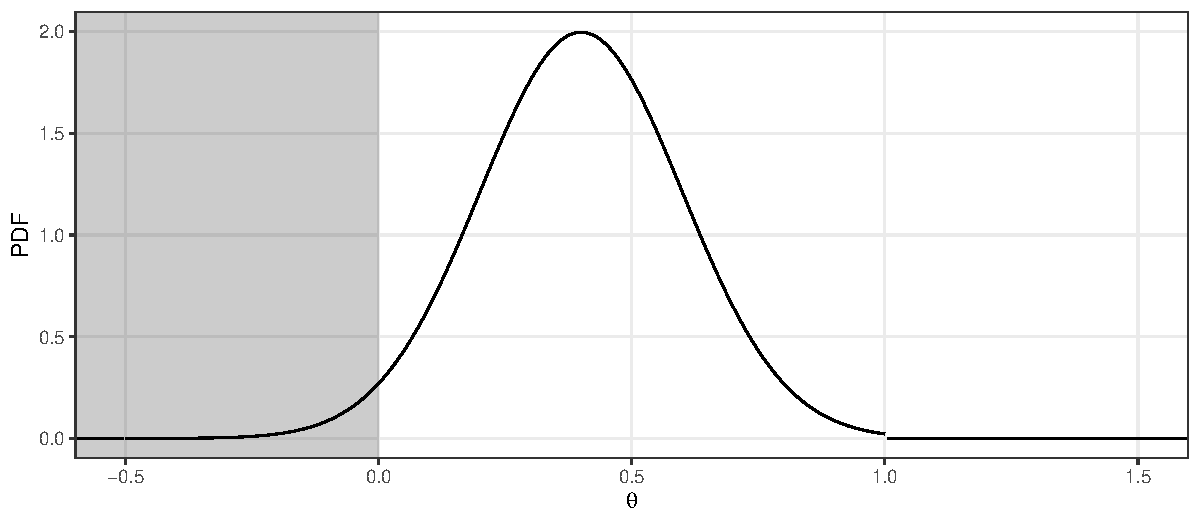
\includegraphics[width=\textwidth]{figures/prior_density}
    \caption{%
        Assumed prior density function.
        The gray area indicates the null hypothesis, $\mathcal{H}_0$, of no effect.
    }
    \label{fig:prior-pdf}
\end{figure}
and that all positive effect sizes are clinically relevant.
A truncated normal prior is convenient since it allows the analytic
computation of the posterior distribution under a normal likelihood.
It is also the maximum entropy distribution on a compact interval given mean and standard deviation and thus "least informative"
given a lower and upper boundary on plausible effects as well as
the location and vagueness (variance) of the prior.
The choice of the prior is a key consideration, but an extensive discussion is beyond the scope of this paper. We refer the reader to discussion in Spiegelhalter \textit{et al.}~\cite{spiegelhalter2004,rufibach_16}, and Hampson \textit{et al.}~\cite{hampson2021}, as well as the formal prior elicitation framework SHELF~\cite{kinnersley2013, shelf}, which is routinely used in practice by pharmaceutical companies~\cite{dallow2018}.

Following~\cite{kunzmann2020} the required
sample size $n$ is determined by requiring
a minimal expected power of $1-\beta=80\%$.
Under these assumptions, the required sample size is
$n = 79$.
Since no point alternative is necessary to derive this sample size, we use the prior mean rounded to the first decimal point to
evaluate $\ACP$ and define $\theta_1:=0.4$.

The three estimators are depicted in Figure~\ref{fig:acp-ocp-pp-comparison-absolute} as functions
of the observed interim outcome, where the interim time-point $m = 26$ (chosen heuristically as approximately 1/3 of the overall sample size).
\begin{figure}
    \centering
    \begin{subfigure}[b]{\textwidth}
        \centering
        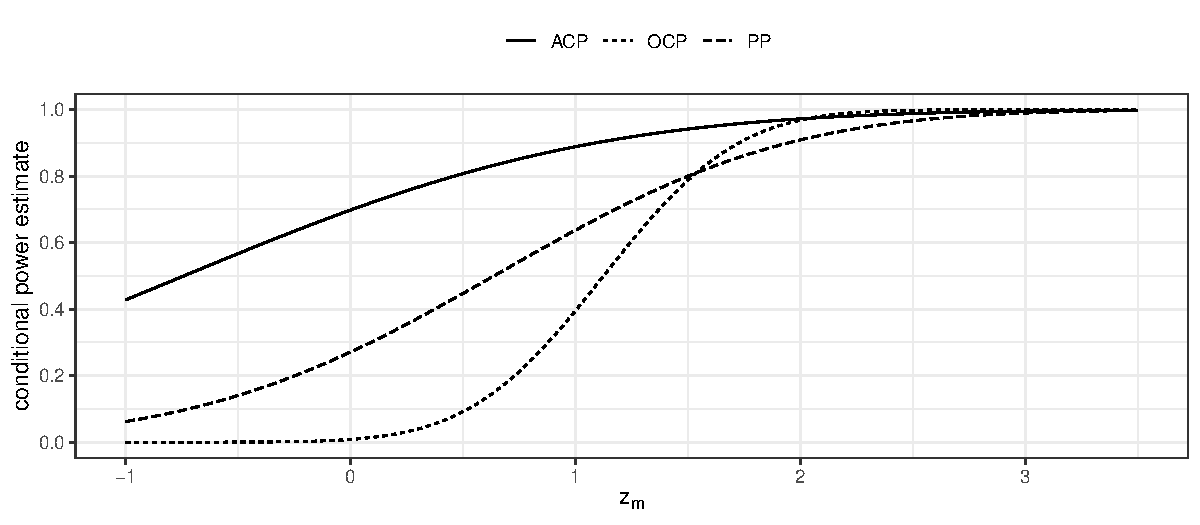
\includegraphics[width=.85\textwidth]{figures/acp_ocp_pp_example}
        \caption{%
            Estimates as function of the interim data.
        }
        \label{fig:acp-ocp-pp-comparison-absolute}
    \end{subfigure}
    \begin{subfigure}[b]{\textwidth}
        \centering
        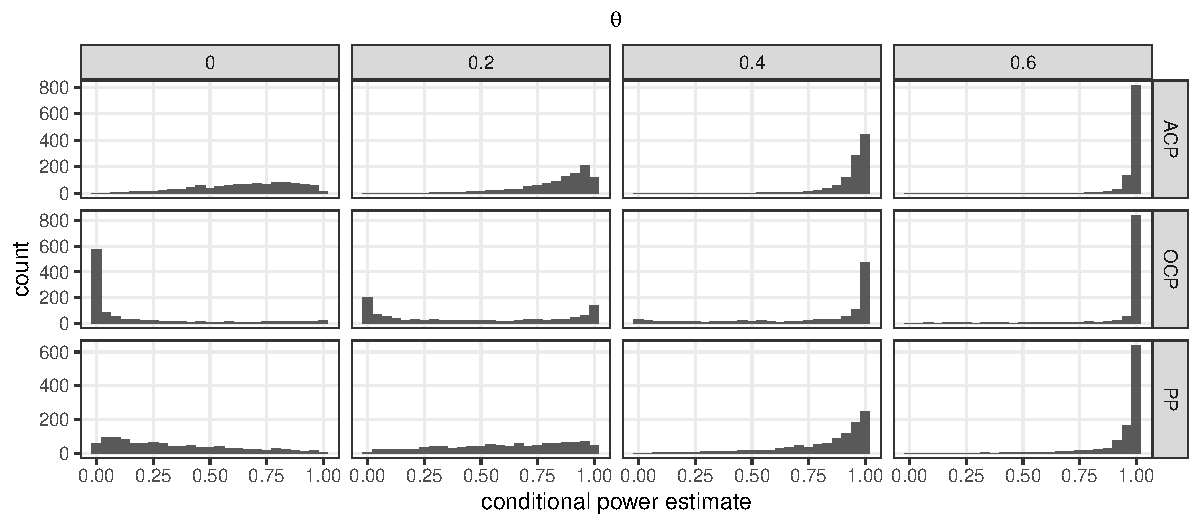
\includegraphics[width=.85\textwidth]{figures/acp_ocp_pp_sampling_distributions}
        \caption{%
            Histograms of the sampling distributions.
        }
        \label{fig:sampling-distributions}
    \end{subfigure}
    \begin{subfigure}[b]{\textwidth}
        \centering
        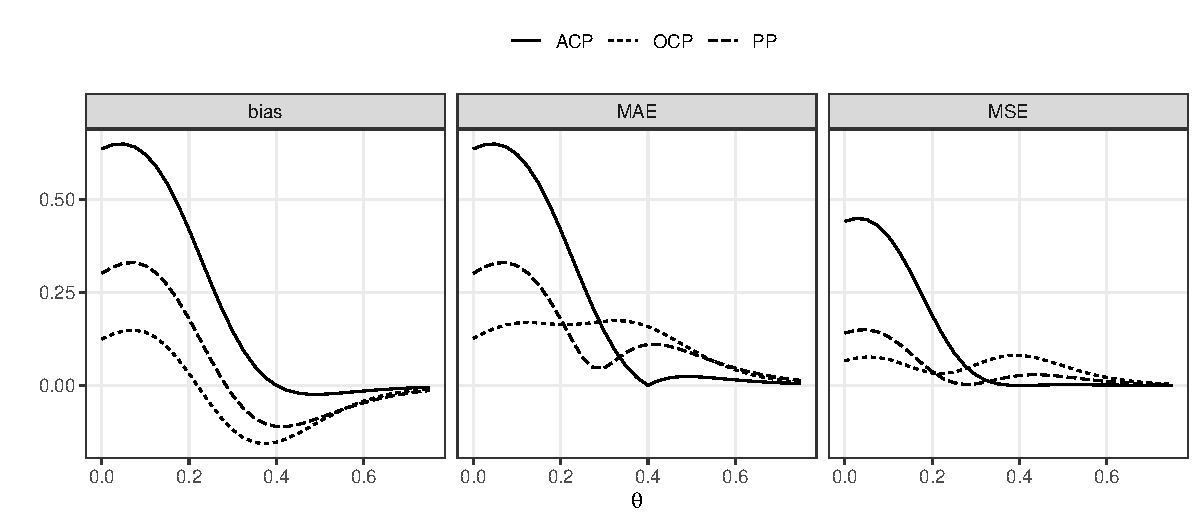
\includegraphics[width=.85\textwidth]{figures/acp_ocp_pp_bias_mae_mse}
        \caption{%
            Bias, mean absolute error (MAE) and mean squared error (MSE).
        }
        \label{fig:acp-ocp-pp-as-estimators}
    \end{subfigure}
    \caption{%
        Properties of $\ACP,\OCP$, and $\PP$ as estimators of the unknown conditional power at $m=26$ and overall sample size $n=79$.
    }
\end{figure}
The most sensitive measure is $\OCP$ while $\ACP$ is the least sensitive
(see also spread of the sampling distributions in Figure~\ref{fig:sampling-distributions}).
This is due to $\ACP$ assuming a fixed effect size and thus
only being affected by direct changes in $z_m$.
Both $\OCP$ and $\PP$, however, are also indirectly affected by updating
the belief about the effect size with the interim results.
The plug-in estimate $\OCP$ assumes that the observed effect is the
true effect and does not quantify the uncertainty around this value in any way.
$\PP$, on the other hand, invokes Bayes' theorem and then integrates
$\CP(z_m,c,\theta)$ with respect to the obtained posterior distribution.
The degree of adaptation of $\PP$ thus depends
on the vagueness of the chosen prior.
In fact, as the prior approaches a point mass at $\theta_1$, $\PP$ converges
to $\ACP$.
$\ACP$ can thus be seen as a mere special case of $\PP$ with a point prior
on $\theta_1>0$.

A fundamental difference between $\ACP$ and $\PP$ on the one hand and $\OCP$ on the other hand is that
$\OCP$ is the only estimator that does not condition on~$\Theta$.
In contrast, $\ACP$ implicitly conditions on $\Theta=\theta_1>0$ and
$\PP$~on~${\Theta > 0}$.
Since $\OCP$ does not condition on $\Theta>0$, the sampling distribution is much more left-skewed for small effects than for the other two estimators (see~Figure~\ref{fig:sampling-distributions}).
Also, the negligence of the sampling variation of $\widehat{\theta}_m$, which $\OCP$ plugs in the expression for conditional power, leads to a larger variance for intermediate values of $\theta$ and the characteristic
U-shape \cite{bauer2006}.
This high variance of $\OCP$ directly translates to a relatively large mean absolute error (MAE) and mean squared error (MSE) when estimating conditional power,
see Figure~\ref{fig:acp-ocp-pp-as-estimators}.
$\PP$ is the posterior expectation of conditional power with respect to the chosen prior (conditional on a positive effect) and thus  minimizes the quadratic Bayes risk, i.e.~the average MSE weighted by $\varphi(\cdot\mid\Theta>0)$.
This leads to relative good precision for parameter values with high \textit{a~priori} likelihood
(around $\theta=0.4$).
If one wanted to minimize the MAE directly,
the posterior median would be optimal.
The principle, however, remains the same and
the posterior mean is more consistent with the derivation of the initial sample size using expected power.
$\ACP$ is clearly the best in terms of bias and MAE/MSE for values close to or
above $\theta_1$, but its performance as estimator of the conditional power
quickly deteriorates for small effect sizes.

$\ACP$ is merely an extreme special case of $\PP$.
$\OCP$ is both hard to justify theoretically and has inferior precision
for parameter values with a high \textit{a~priori} likelihood.
$\PP$ is thus the natural choice for monitoring power during the course of a trial.
Depending on the prior chosen, its properties can be either more similar to $\ACP$ (low prior variance) or $\OCP$ (high prior variance).



\subsection{Na\"{\i}ve unplanned sample size adaptations}
\label{sec:naive-adaptations}

Monitoring the predictive power of an ongoing trial naturally raises the question of whether this information can be leveraged to improve the operating characteristics of a trial.
Typically, sample size recalculation is considered in the context of group-sequential designs at the pre-specified interim analysis \cite{proschan1995,brannath2004,bauer2016}.
From a statistical perspective, however,
there is no reason why a sample size recalculation should not be
performed for a study that initially was planned using a single-stage design.
For the sake of simplicity the following considerations are based on a single-stage design with fixed $n$ and $c$ as starting point.
We restrict the discussion to a single unplanned interim analysis.
All results can be generalized to the case of more complex starting designs and multiple interim analyses.

A method for sample size recalculation that is often discussed in the literature is to derive a new sample size $n'$ and a new critical value $c'$ such that some estimate of conditional power exceeds a threshold $1-\widetilde{\beta}(z_m)$ that may or may not vary with the observed interim result.
Different choices for the estimator of conditional power
and the choice of $\widetilde{\beta}(z_m)$ have been discussed in the literature \cite{proschan1995,brannath2004,bauer2016}.
Strict overall type~I error rate control can be maintained by invoking the conditional error principle \cite{muller2001,muller2004,brannath2012}, i.e., by limiting the maximal type~I error rate of the new design to the maximal conditional type~I error rate of the original design given the observed $z_m$.
Often, trial protocols leave the exact choice of $1-\widetilde{\beta}(z_m)$ open since it can be chosen \textit{ad~hoc}
without compromising strict type~I-error rate control.
The basic concept of adjusting the sample size to achieve the desired conditional power is, however, a common approach, see for instance Bhatt~\etal~\cite{bhatt2013} and~Mehta~\etal\cite{mehta2009}.

In accordance with the discussion in the previous section
and to be consistent with the derivation of the
initial sample size of $n=79$ in the example considered earlier,
we use predictive power as an estimator of conditional power.
Furthermore, we set $\widetilde{\beta}(z_m)=\beta=0.2$.
For given $Z_m = z_m$, the recalculation rule then corresponds to solving
the optimization problem
\begin{align}
    \argmin{n', c'} &&                   n' & \label{eq:naive-recalc}\\
    \st             && \CP(m, n', z_m, c', 0) &\ \leq \ \CP_n(m, n, z_m, c, 0) \label{eq:ce-principle-naive-recalc} \\
                    &&    \PP_\varphi(m, n', z_m, c') &\ \geq \ 1 - \widetilde{\beta}(z_m) \\
                    &&                   n' &\ \geq \ n_{min} > m \label{eq:nmin-naive-recalc} \\
                    &&                   n' &\ \leq \ n_{max} \label{eq:nmax-naive-recalc} \ .
\end{align}
Here, we indicate the dependency on the
final sample size and the interim time point explicitly by redefining
\begin{align}
    \CP(m, n, z_m, c, \theta) :&= \Pr_\theta[\,Z_n > c \cond Z_m = z_m\,] \\
    \PP_\varphi(m, n, z_m, c) :&= \Pr_\varphi[\,Z_n > c \cond \Theta >0, Z_m = z_m\,] \ .
\end{align}
Constraint~\eqref{eq:ce-principle-naive-recalc} implements the conditional
error principle by limiting the conditional (type~I) error rate under the new design to
the conditional (type~I) error rate under the original design.
The minimal sample size constraint~\eqref{eq:nmin-naive-recalc} allows  $n_{min}>m$ for cases where a minimal sample size upon rejection of the null hypothesis is deemed necessary.
Note that the trial cannot stop at $n'=m$ without immediately accepting the
null hypothesis since the conditional error under the new design in the case of early acceptance would be $1$ but is always smaller than $1$ for the original single-stage design.
Imposing a maximal sample size of $n_{max}$ via constraint~\eqref{eq:nmax-naive-recalc} is a practical necessity since the
recalculated sample size could otherwise tend to infinity as $z_m$ approaches negative infinity.
In cases where this constraint prevents a solution (low observed effect),
the trial is usually stopped early for futility declaring that the null hypothesis cannot be rejected.

If the recalculation rule defined in \eqref{eq:naive-recalc}--\eqref{eq:nmax-naive-recalc} is made mandatory in the
study protocol,
it yields two functions $n(z_m)$ and $c(z_m)$ as the point-wise solution of the problem
which jointly define an adaptive design.
Here, "mandatory" means that it is decided \textit{a~priori} to always (for all $z_m$)
recalculate the
final sample size and critical value in the
above specified way after a fixed number of outcomes $m$ has been observed.
The term "adaptive design" is slightly misleading in this context.
The design itself is pre-specified (and thus not adapted or changed)
but only $n$ and $c$ are adaptive since they vary as functions of $z_m$.
The corresponding sample size and critical value functions for $m=26$ are depicted in Figure~\ref{fig:binding-recalculation}.
\begin{figure}
    \centering
    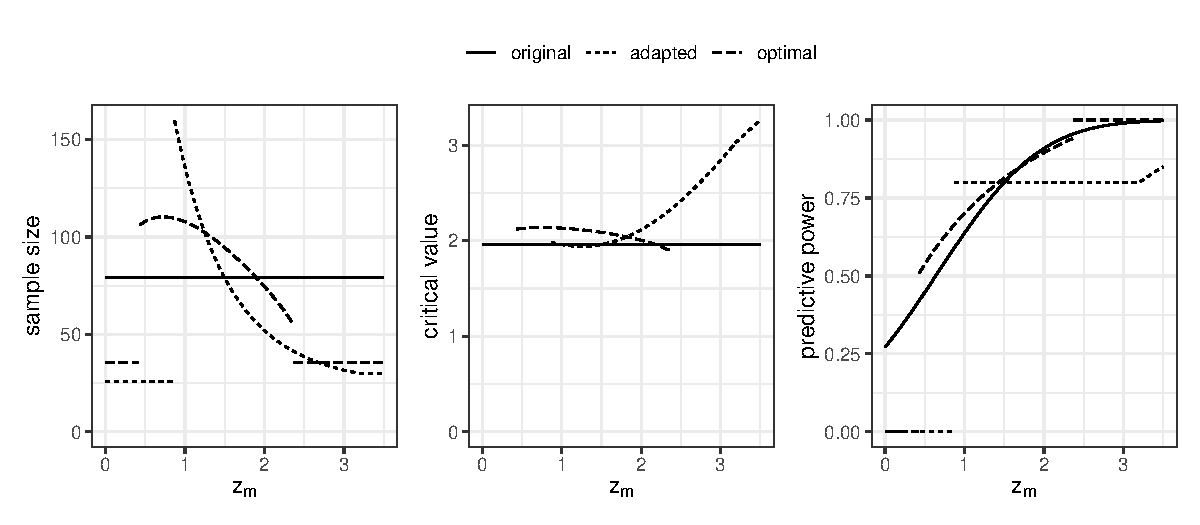
\includegraphics[width=\textwidth]{figures/naive_adaptive_and_optimal_designs}
    \caption{%
        Original single-stage design; na\"{\i}vely adapted design
        with sample size $n'(z_m)$ and critical value $c'(z_m)$ functions defined by the conditional optimization problem \eqref{eq:naive-recalc}--\eqref{eq:nmax-naive-recalc} and
        ${n=79}, {m=26}, {n_{max}=160}, {n_{min}=30}$ and $1-\widetilde{\beta}(z_m)=0.8$;
        the optimal design is the solution of \eqref{eq:optimal-design-start}--\eqref{eq:optimal-design-end}.
    }
    \label{fig:binding-recalculation}
\end{figure}

The mandatory application of the adaptation rule
results in a two-stage design and the final sample size is thus a random variable $n(Z_m)$.
Optimality can thus no longer be defined in terms of the (random) sample size itself but only in terms of a functional of the distribution of $n(Z_m)$.
For instance, one could use a weighted sum, $\E[\,n(Z_m)\,] + \eta \sqrt{\V[\,n(Z_m)\,]}$, of the expected value and standard deviation of the sample size as the objective criterion.
The rationale for adding a penalty depending on the standard deviation of the sample size is that it might incur additional costs due to more
complicated logistics (e.g., on demand production of additional drug doses).
For the single-stage design this proposal always reduces to the fixed sample size $n$.
Whether or not the two-stage design is considered better then depends on the choice of $\eta$ (the relative weight of the the standard deviation in the objective).
In the particular situation considered here, the expected sample size is $48.3$ and its standard deviation is $30.1$.
Since the original $n$ was $79$, the two-stage
design would be considered better
than the single-stage design for $\eta<1.02$.

This comparison ignores the fact that
the original unconditional constraint of an expected power of more than $80\%$
is no longer fulfilled by the design with mandatory
sample size adaptation.
Both expected power ($66.9\%$ \emph{versus} $80.0\%$) and maximal type~I error rate ($1.8\%$ \emph{versus} $2.5\%$) are lower than for the original design.
The difference in operating characteristics is mainly due to the fact
that the new design implicitly introduces a binding early-stopping boundary for futility
when the recalculation problem does not yield a $n'\leq n_{max}$.
Similar to suggestions in the literature on binding futility stopping,
one could modify the initial nominal $\alpha$ and the conditional power threshold $\widetilde{\beta}(z_m)$ until the recalculated design again fulfills the required
operating characteristics \cite{brannath2004}.
This approach to define a fully pre-specified two-stage design is, however, unnecessarily complicated in that it
uses methods which are originally intended for \emph{unplanned}
design adaptations and that
they still implicitly depend on a design that is never actually realized via the
conditional error constraint~\eqref{eq:ce-principle-naive-recalc}.



\subsection{Optimal pre-planned sample size adaptations}
\label{sec:optimal-adaptation}

Instead, the interim time-point $m$,
the sample size function $n(z_m)$,
the critical value function $c(z_m)$,
and the early futility- and efficacy boundaries
($n(z_m)=m$ and $ c(z_m)=\pm\infty$)
can be optimized directly.
For the sample size function $n(z_m)$ Brannath~\textit{et al.}~\cite{brannath2004} discussed this approach by fitting a polynomial of degree 4 but they did not optimize
any of the other parameters.
Pilz~\textit{et~al.}~\cite{pilz2019} approached the problem in a more general form using
variational methods.
An \texttt{R} implementation that uses cubic splines for both the $n$ and
$c$ functions is available via the package~\texttt{adoptr}~\cite{adoptrjss2020}.

In the following we restrict the considerations to the case
where only expected sample size is of interest and the variability of the sample size is
ignored, i.e.~$\eta=0$.
The corresponding optimal two-stage design is the solution of
\begin{align}
    \argmin{m, n(\cdot), c(\cdot)}
        &&                                   \E_\varphi[\,n(Z_m)\,] & \label{eq:optimal-design-start}\\
    \st &&                 \Pr_{0}[\,Z_{n(Z_m)} > c(Z_m)\,] & \leq \alpha \\
        &&     \EP_\varphi\big(n(\cdot), c(\cdot)\big) & \geq 1 - \beta \label{eq:optimal-design-end}
\end{align}
and can be derived numerically using the \texttt{R} package \texttt{adoptr}~\cite{adoptrjss2020}.
In the following, "optimal" always refers to optimal with respect to expected sample size in the above sense.
Here, $\E_\varphi[\,n(Z_m)\,]$ is the expected sample size under the prior $\varphi$ and expected power needs to be redefined to account for the
fact that $n$ and $c$ are now functions of the interim results
\begin{align}
    \EP_\varphi\big(n(\cdot), c(\cdot)\big) :=
    \Pr_\varphi\big[\,Z_{n(Z_m)}>c(Z_m)\,|\,\Theta>0\,\big] \ .
\end{align}
Figure~\ref{fig:binding-recalculation} shows the sample size-, critical value-, and the predictive power function in the situation discussed earlier together with the single-stage design
and the na\"{\i}ve adaptation based on predictive power discussed in
Section~\ref{sec:naive-adaptations}.
The optimal two-stage design complies with both the predictive power and the maximal type~I error rate constraints and is thus comparable with the original single-stage design in terms of sample size.
The expected sample size is much lower ($56.4$ \emph{versus} $79$) at the cost of a non-zero standard deviation of the expected sample size ($28.5$ \emph{versus} $0$).
Since it is entirely pre-specified,
the optimal two-stage design does not need to fall back to the conditional error principle to control the maximal type~I error rate.
Instead, it achieves the desired design characteristics in an optimal way since they are incorporated as constraints to problem \eqref{eq:optimal-design-start}--\eqref{eq:optimal-design-end}.
The optimal design fully exhausts the allowable maximal type~I error rate
and complies with the expected power constraint.
This comes at the cost of a predictive power that can drop as low as 40\% close to the futility boundary
as shown in the right panel of Figure~\ref{fig:binding-recalculation}.
The sample size function of the optimal design is also
characteristically different from the na\"{\i}ve design.
The latter is convex on the continuation region whereas the optimal
shape has a mode close to the early-futility boundary.
A~recalculation based on exceeding a fixed lower threshold for
some estimator of conditional power always results in a convex
sample size function and can thus never be fully optimal irrespective of how the nominal values of $\alpha$ and $\widetilde{\beta}(z_m)$
are chosen.
For a more detailed discussion of this phenomenon see~e.g.~\citep{pilz2019,brannath2004}.

The fact that the optimal two-stage design exhibits a monotonously increasing
predictive power rather than a constant predictive power
indicates that any recalculation rule keeping predictive power
close to a fixed target value must be inefficient in terms of minimizing expected sample size.
The mandatory application of the heuristic recalculation rule introduced in Section~\ref{sec:naive-adaptations} would change the optimal design for almost every value of $z_m$ and thus increase expected sample size
of the resulting design.
This is inconsistent with the original optimization objective -
by definition,
no optimal design ever needs to be changed as a reaction to trial internal data alone during the course of the study.
The direct optimization of all design parameters is superior to the mandatory application of methods for unplanned design adaptations during the planning phase of a trial.
However, there are still situations in which an unplanned sample size recalculation is warranted.
The optimality of a design typically depends on the chosen prior density $\varphi$ and the objective function.
At any point in time,
the prior density encodes all trial-external evidence
about the effect size.
This might change over the course of a trial.
For instance, another study might publish new results that trigger a reassessment of the considerations leading to the choice of $\varphi$.


\section{Consistent unplanned sample size adaptations}
\label{sec:unplanned-adaptation}

In the following, we discuss two approaches of reacting to
trial-external events during an unplanned interim analysis in a consistent way.
Here, "consistent" means that the original design is invariant under
the sample size recalculation rule for all potential interim
results under the original design unless the planning assumptions or
the time-point of the interim analysis are changed.
An example for such an inconsistent sample size recalculation rule was given in Section~\ref{sec:naive-adaptations}:~The design optimizing expected sample size is not invariant under a rule that adapts the sample size and the critical value to match a predictive power of exactly $80\%$.
The same holds for a simpler group-sequential design minimizing expected sample size
since the predictive power of a group-sequential trial cannot be constant on the continuation area.
The following considerations are restricted to cases where the result of an adaptation is a final sample size and no further interim analyses are planned for the remainder of the trial.
This means that the unplanned adaptation replaces the pre-planned interim analysis although it might occur at a different point in time.

We consider minimal expected sample size as original objective criterion.
Since the sample size after the interim analysis is fixed,
the corresponding conditional objective criterion is the minimization of the second-stage sample size.
As in Section~\ref{sec:naive-adaptations}, the overall type~I error rate is controlled via a
constraint on the conditional type~I error rate.
W.l.o.g.,~we only consider cases where the original design would not stop early for futility or efficacy.
Let $\psi$ be the probability density function of the revised prior.
We propose to recalculate the new sample size $n'$ and
the new critical value $c'$ as the solution of the point-wise (conditional on $Z_{m'} = z_{m'}$) optimization problem
\begin{align}
    \argmin{n',c'} && n' & \label{eq:objective-original-interim}\\
    \st
    && \CP(m, n', z_{m}, c', 0) &\leq \CP(m, n(z_m), z_{m}, c(z_m), 0) \\
    && \PP_\psi(m, n', z_{m}, c') &\geq 1 - \widetilde{\beta}(z_m) \ . \label{eq:objective-original-interim-end}
\end{align}
Since $\CP$ is monotone in $n'$, the solution is uniquely
defined by the constraints, if it exists.
The optimization thus reduces to finding the root of
\begin{align}
    \solve{n',c'} \qquad
    & \CP(m, n', z_{m}, c', 0) &&= \CP(m, n(z_m), z_{m}, c(z_m), 0) \label{eq:root-cp}\\
    & \PP_\psi(m, n', z_{m}, c') &&= 1 - \widetilde{\beta}(z_m) \ . \label{eq:root-pp}
\end{align}
The central problem is translating the unconditional (expected) power constraint of the
original design problem into a conditional one for predictive power - i.e.~to pick a value for $\widetilde{\beta}(z_m)$ - in a way that ensures consistency of the recalculated sample size and critical value with the original design if neither the interim timing nor the planning assumptions change.
As discussed in Section~\ref{sec:naive-adaptations}, a constant value for $\widetilde{\beta}(z_m)$ does not, in general, lead to a consistent recalculation rule.
Below, we propose two consistent recalculation rules,
both are based on an application of the conditional error principle to the (expected) type~II error rate.
The first rule does not require knowledge of the underlying optimization problem for the original design.
This approach is easy to implement but does not maintain the unconditional power properties of the design, which is addressed by the second proposal.


\subsection{"Not-worse" approach}
\label{sec:not-worse}

A sensible heuristic criterion to chose $\widetilde{\beta}(z_m)$ is to require that the modified design under the new prior $\psi$ should have at least as much predictive power as the original design under the original prior $\varphi$,
i.e.~$\widetilde{\beta}(z_m) = {1 - \PP_\varphi(m, n(z_m), z_{m}, c(z_m))}$.
Consequently, we term this choice of $\widetilde{\beta}(z_m)$ the "not-worse" approach.
It follows that, for $\psi=\varphi$,
the original design's $n(z_m)$ and $c(z_m)$ are a root of \eqref{eq:root-cp}-\eqref{eq:root-pp} and hence ${n'=n(z_{m})}$, ${c'=c(z_m)}$.
The original optimal design is thus indeed invariant under the
proposed recalculation rule if neither the planning prior nor the interim time-point are changed.
However, the
expected power of the procedure resulting from always switching to
a new prior $\psi\neq\varphi$ will be different from the originally targeted $1-\beta$ since $1-\widetilde{\beta}(z_m)$ does not integrate to $1 - \beta$ under~$\psi\neq\varphi$.
To see this, let $f_\psi(z_m \mid \Theta>0)$ be the probability density function of the interim result $Z_m$ under $\theta\sim\psi$ conditional on $\Theta>0$, then
{\small
\begin{align}
    \EP_\psi\big(n'(\cdot), c'(\cdot)\big) &=
    \Pr_\varphi\big[\,Z_{n'(Z_m)}>c'(Z_m)\,|\,\Theta>0\,\big]  \\
    &= \int \PP_\psi(m, n'(z_m), z_{m}, c'(z_m)) \ f_\psi(z_m \mid \Theta > 0) \operatorname{d} z_m \\
    &= \int \underbrace{\big(1 - \widetilde{\beta}(z_{m})\big)}_{\PP_\varphi(m, n(z_m), z_{m}, c(z_m))} \ f_\psi(z_m \mid \Theta > 0) \operatorname{d} z_m \\
    &\neq \int \PP_\varphi(m, n(z_m), z_{m}, c(z_m)) \ f_\varphi(z_m \mid \Theta > 0) \operatorname{d} z_m \\
    &= \EP_\varphi\big(n(\cdot), c(\cdot)\big) = 1 - \beta \ .
\end{align}}



\subsection{"Reoptimization" approach}
\label{sec:reoptimize}

To additionally maintain the unconditional (expected) power during an unplanned sample size recalculation,
$1-\widetilde{\beta}(z_m)$ needs to integrate to $1-\beta$ under the modified prior $\psi\neq\varphi$.
We propose to achieve this with a two-step procedure.
Firstly, a modified version of the original optimization problem \eqref{eq:optimal-design-start}-\eqref{eq:optimal-design-end} is solved where the original prior~$\varphi$ is replaced with the updated prior~$\psi$,
and under the additional conditional type~I error rate constraint dictated by the conditional error principle, i.e.
{\small\begin{align}
    \argmin{n''(\cdot), c''(\cdot)}
        &&                                   \E_\psi[\,n''(Z_m)\,] & \\
    \st &&                 \Pr_{0}[\,Z_{n''(Z_m)} > c''(Z_m)\,] & \leq \alpha \\
        &&     \EP_\psi\big(n''(\cdot), c''(\cdot)\big) & \geq 1 - \beta \\
        && \CP(m, n''(z_{m}), z_{m}, c''(z_{m}), 0) &\leq \CP(m, n(z_m), z_{m}, c(z_m), 0) \label{eq:cp-reoptimize}
\end{align}}

\noindent One could use $n''(z_m)$ as recalculated sample size and the corresponding critical value~$c''(z_m)$ directly.
However, there may be cases where the conditional type~I error rate constraint \eqref{eq:cp-reoptimize} is not binding leading to an unnecessarily low conditional error and thus a needlessly large sample size.
Instead, as the second step, we propose to plug in  $1-\widetilde{\beta}(z_m)=\PP_\psi(m, n''(z_m), z_{m}, c''(z_m))$ in \eqref{eq:root-cp}-\eqref{eq:root-pp} and solve for $n'$ and $c'$.
Since,
{\small
\begin{align}
    1-\beta &\leq\EP_\psi\big(n''(\cdot), c''(\cdot)\big) \\
    &= \int \underbrace{\PP_\psi(m, n''(z_m), z_{m}, c''(z_m))}_{1-\widetilde{\beta}(z_m)} \ f_\psi(z_m \mid \Theta > 0) \operatorname{d} z_m \ ,
\end{align}}

\noindent the \emph{unconditional} expected power of the recalculation procedure maintains the original value of $1-\beta$.
Note that this only holds true if the choice of~$\psi$ is stochastically independent of $Z_m$, i.e.~if the change of the planning assumptions is not driven by the observed interim data.

\subsection{Application Example}
\label{2arm}

In practice, group-sequential designs are more common than optimal two-stage designs.
Since the efficiency gains of the latter over the simpler group-sequential designs
are often practically irrelevant this is a sensible approximation~\citep{wassmer2016}.
Sample size calculations are still commonly based on point alternatives.
This is equivalent to using a point prior on the alternative value.
All previous considerations can thus be transferred to a setting with a fixed
point alternative.

For this example, we consider the two-stage, two-arm group-sequential design with binding early stopping for futility boundary at an observed effect of $0$ that minimizes the expected sample size under the point alternative of a mean difference of $\theta_1=0.4$ under a one-sided type~I error rate constraint of $\alpha \leq 0.025$ and  an expected power of at least $0.8$.
Since the prior only has mass at $\theta_1=0.4$ this corresponds to a classical power constraint at $\theta_1=0.4$.
We computed the optimal group-sequential design by direct minimization over the stage-one and two sample sizes and the stage-two critical value using the \texttt{R}~package \texttt{nloptr}~\cite{nloptr}.

We first consider a scenario where the alternative is modified during the interim analysis to either $\theta_1=0.35$ or $\theta_1=0.45$ \emph{independently} of the
observed interim data.
The conditional and unconditional properties of three adaptation procedures together with those of the original design are shown in Figure~\ref{fig:application-example-1}.
Firstly, "PP >= 0.8" corresponds to a recalculation based on a fixed threshold for the predictive power of $0.8$.
As discussed earlier, this adaptation rule is not consistent in that the original design is not invariant under recalculation (see Section~\ref{sec:naive-adaptations}).
Secondly, the "not-worse" approach discussed in Section~\ref{sec:not-worse} instead matched the predictive power of the original design under the old prior.
Thirdly, the "reoptimize" approach discussed in Section~\ref{sec:reoptimize} matches the predictive power of design that is optimal under the new alternative.
For all recalculations, the final adapted sample size was restricted to the range of $120$ to $400$.
\begin{figure}
    \centering
    \includegraphics[width=\textwidth]{figures/application-example}
    \caption{%
        Left: Sample size (both arms) and predictive power for response-independent adjustment of the alternative; predictive power is evaluated at the respective changed point alternative.
        Right: unconditional (expected) power and expected sample size for the three scenarios when adapting to the respective true $\theta$ (for $\theta=0.4$, the two consistent rules overlap with the original design).
    }
    \label{fig:application-example-1}
\end{figure}
Clearly, "PP >= 0.8" is not only inconsistent but also the rule that leads to the most extreme adaptation of the sample size.
The "not-worse" approach leads to a level-shift in the sample size with moderate
increases or decrease of the stage-two sample size.
The "reoptimize" approach leads to more moderate increases in sample size
as compared o the "PP >= 0.8" approach when the alternative is lowered and to substantial sample size reductions for an increased effect size.
From an unconditional perspective, only the "reoptimize" approach maintains the target expected power of $0.8$.

A conceptual drawback of point priors is that they are invariant under
formal Bayesian updating.
This means that the posterior distribution after observing the interim results
is always the same point measure as the initial point prior
and is merely a consequence of claiming perfect knowledge of the effect size during planning.
In practice,
investigators might still be inclined to modify the alternative at least heuristically during the interim analysis.
We thus consider an alternative situation based on the same optimal group-sequential design discussed above.
Assume that the trial team wants to revise the strong assumption of a point prior on the alternative of a mean difference of $0.4$ during the interim analysis using the observed interim data.
For instance this could be done heuristically by "updating" the alternative to the average of the observed effect and the originally assumed point alternative of $0.4$.
The resulting conditional and unconditional properties of the proposed recalculation rules are given in Figure~\ref{fig:application-examplel-response-adaptive}.
\begin{figure}
    \centering
    \includegraphics[width=\textwidth]{figures/application-example-response-adaptive.pdf}
    \caption{%
        Left: Sample size (both arms) and predictive power for response-adaptive modification of the alternative; predictive power is evaluated at the respective changed point alternative.
        Right: unconditional (expected) power and expected sample size for three scenarios.
    }
    \label{fig:application-examplel-response-adaptive}
\end{figure}
In this alternative scenario, the adapted sample size under all three rules is more variable and quickly reaches the maximal value of $400$.
In this scenario, the sample size is rarely reduced since the original group-sequential design employs an aggressive early-efficacy boundary of $\approx 0.4$ on the scale of the observed treatment effect.
Hence, the heuristically modified alternative almost never exceeds the original value of $\theta_1 = 0.4$.
Since the adaptation is now response-adaptive, the "reoptimize" approach does no longer maintain a power of $1-\beta$.

These two example situations show that a consistent sample size adaptation can make sense as reaction to new trial-external evidence.
For the relevant case of reacting to new trial-external evidence,
it is possible to maintain the unconditional power properties of the original design.
If, however, the change of alternative depends on the observed interim data,
it is unclear how the unconditional power may be preserved.


\section{Discussion} %%%%%%%%%%%%%%%%%%%%%%%%%%%%%%%%%%%%%%%%%%%%%%%%%%%%%%%

Monitoring the power of the remainder of an ongoing trial constitutes an estimation problem since the conditional power
is a function of the unknown treatment effect.
This estimation problem can be formulated both conditional or unconditional on a positive treatment effect.
In many practical situations where the prior mass is concentrated on non-null effects the consequences of conditioning are negligible but their importance increases with the vagueness of a the prior.
The lack of conditioning on a positive treatment effect explains why observed conditional power performs rather poorly as an estimator of the unknown conditional power for a wide range of effect sizes.
Assumed conditional power for $\theta_1>0$ does reflect this conditionality.
It is, however,
merely a special case of predictive power with a
point prior on the effect size.
In situations where the effect size is fairy well known, a point prior might constitute an acceptable, simpler approximation.
In any other case, the Bayesian predictive power allows \textit{a~priori} information to be incorporated in a more fine-grained way and
guarantees optimal mean-squared-error performance.
If an unconditional measure for the probability to reject the null hypothesis is sought,
a conditional version of the probability of success (or assurance) can be derived in an analogue way~\cite{kunzmann2020}.

Great care should be taken when predictive power
or another estimator of conditional power
is used to modify an ongoing trial's sample size.
Altering a simple starting design with a seemingly intuitive recalculation rule
can lead to overall \emph{less effective} trials.
Techniques originally intended for \emph{unplanned} adaptations of trials
should not be used for a \emph{pre-planned} sample size recalculation.
Instead, an optimal two-stage design should directly be derived
for the objective criterion of interest.
By definition, no trial-internal event can then justify a sample size recalculation.
Only trial-external events, such as a change in the objective criterion,
the emergence of new trial-external evidence,
or unforeseen deviations from the planned interim analysis time-point
may require a reassessment of the sample size of an optimal design.

A~generic recalculation rule might lead to the paradoxical situation that an optimal
starting design is always modified during the interim analysis
- even if the planning assumptions remain unaltered throughout the trial.
This is clearly ineffective and, consequently,
an optimal starting design should be invariant under a sensible adaptation rule
if the planning assumptions remain unchanged.
This minimal consistency property is often not fulfilled when recalculating a design's
sample size based on a fixed threshold for its minimal conditional power.

We proposed two consistent approaches to adjusting an ongoing optimal design to
newly emerging trial-external data.
Both methods can be extended to deviations from the planned interim time-point.
The first method ("not-worse") applies the conditional error principle to the (average) type~II error rate in a similar way to its use in controlling the maximal type~I error rate.
The method is easy to implement and consistent in the above defined way.
However, it does not maintain the same unconditional power as the original design,
not even under data independent modifications of the planning assumptions.
The second method addresses this issue by adapting the sample size and critical value such that the predictive power matches the predictive power of a design that would have been optimal, had the new prior been known during the planning stage.
As long as the prior is adapted data-independently, this approach does indeed maintain the same unconditional power properties.

These considerations show how crucial the initial planning stage of a trial is.
Adaptive methods should not be taken as an excuse to start with a
sub-optimal design and rely on a later sample size recalculation.
Ideally, all uncertainty is quantified during the planning phase to
the best possible extent and integrated in the initial design via a
planning prior.
A modification of the design is then only necessary and warranted
when this planning prior changes.
This does not mean that a complex design is always the best choice.
If the variability of the final sample size and the operational
burden of conducting interim analyses is penalized strong enough in
the objective criterion, a simple one-stage design might very well
perform better than more complex alternatives.
Generic optimal-two stage designs require optimizing over function-spaces to find the optimal sample size and critical value functions.
Obtaining a stable solution might thus be hard in practice and
group-sequential designs are a viable approximation since optimizing the stage-wise sample sizes and stopping boundaries only requires optimizing over a small set of real parameters.
It is well-known, that optimal group-sequential designs approximate the performance of optimal two-stage designs with variable sample sizes sufficiently well~\cite{wassmer2016}.
Still, the same principle considerations apply:
An optimal (group-sequential) design only needs to be revised if either the objective function or the underlying planning assumptions, i.e.~the prior on the effect size, changes.

A limitation of the proposed recalculation methods is the fact that they
rely on the conditional error principle for strict type~I-error rate control.
The conditional error principle can be difficult to extend to cases with nuisance
parameters \cite{gutjahr2011}.
In practice, a simple plug-in approach similar to the approach in blinded sample size reassessment might be viable but has not yet been investigated more thoroughly.
Alternatively, any other form of pre-specifying a combination function for the stage-wise $p$-values might be used to control the type~I-error rate.
This combination function should then also be optimized over during the planning stage
to avoid inconsistencies.
In particular, the optimal combination function of a two stage-design minimizing expected sample size can be approximated with an inverse normal combination test~\cite{pilz2019}.

\subsection*{Acknowledgments}

We would like to thank the editor and an anonymous reviewer for their excellent comments which greatly improved the manuscript.

\subsection*{Data Availability Statement}

The source code required to reproduce all results presented in this manuscript is available at
\href{https://github.com/kkmann/unblinded-sample-size-adaptation}{github.com}
and
\href{https://doi.org/10.5281/zenodo.3925752}{zenodo.org}.

\subsection*{Funding}

This research was supported by the NIHR Cambridge Biomedical Research Centre (BRC-1215-20014). The views expressed are those of the authors and not necessarily those of the NHS, the NIHR or the Department of Health and Social Care. David S.\ Robertson was funded by the Biometrika Trust and the Medical Research Council under Grant MC\_UU\_00002/6.


\bibliography{manuscript.bib}

\end{document}
